\subsection{Your site should look good}

You want to grab the users attention from the outset - it is important that the information is attractive and eye-catching.
This is important not only from an aesthetic point of view, but also from a functional one.
This is similar to the importance of good data presentation, using a structure that guides the user in a logical and orderly manner.\\

Other more technical characteristics are:
\begin{itemize}
    \item\textbf{Consistent} Controls that perform similar actions should have the similar appearance.
    A label with different typology or other color may jar the user's perception. Use strong colours sparingly, when
    you want to highlight something in particular. \\

    \item\textbf{Clean and well-organized} An organized design looks better, give a more peaceful feeling and enables the user to find what they are looking for more easily. \\ 

    \item\textbf{Branded} It is highly recommended to 'brand' yourself, so that users can recognize you quickly. For this you can utilize a symbol, a combination of colours, a logo, or a device.
    All the value arising from the quality of your product will accrue to your brand. It is an asset that can be reused in other contexts. \\
\end{itemize}

% TODO: Not sure where this belongs. Maybe compelling?
% To be able to hook our users, gamification is currently widely used. This is where we give a gaming aspect to the representation of the data. The user tries it because it catches their attention, it's fun.
% Certainly, at some point the novelty wears off, but, even so, the user has learned to use the interface and now feels well-disposed to continue to use it.

\subsubsection*{Suggested strategies}

\begin{itemize}
    \item To make an attractive design, we must keep abreast of current trends, and study good design practices.
    \item Maintain a simple and clean design, and use standards and mechanisms that are familiar to users.
\end{itemize}

\subsubsection*{In the context of Aire Guru \ldots}

The visual design of Aire Guru is based on Google's Material Design, using straight lines, differentiating individual sections by using rectangles
and using colours that contrast the information from the background.
The background color for the graphics is a neutral white.
Only shades of blue, grey and white are used. In addition, we chose a font that is easy to read.\\

The sections are arranged neatly and regularly, and structured by using a header and a body.\\

The central page consists of a header, the body and a footer. Both the header and the footer are static,
they are shown in all the pages and they contain all the information needed to navigate between pages. Thus the site controls are consistent no matter what page the user is on.
The body is divided into three horizontal sections, the upper area with the map and the general information about the selected point,
the central area where we can filter the pollutants by medical conditions and information about the current air status, and the
lower area where we have the zone and custom history.\\

\begin{figure}[ht]
    \centering
    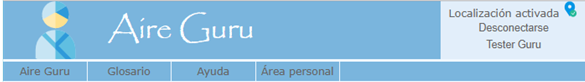
\includegraphics[width=12cm]{Figure_6_6_1_heading}
    \caption{Heading}
\end{figure}

\begin{center}
    \bf{     
    Figure 6.6.1. Heading}
  \end{center} 
 
The symbol of our website is a genius - a guru. We also include the word "Aire" in the logo, because it perfectly represents 
what we show with our website. Aire, as you might have guessed, is Spanish for Air. Aire Guru is the guru of air quality. \\

Finally, we've taken into account that the user may wish to use our website on different devices, therefore we have implemented
two different formats, one for larger screens such as the computer and another for smaller format tablets or mobile devices.